\documentclass[a4pa<per,12pt,spanish]{article}
\usepackage{colortbl}
\usepackage[dvipsnames,table]{xcolor}
\usepackage{booktabs}
\usepackage{tabularx}
\usepackage[headsep=0.2cm,headheight=1.5cm,left=2cm,right=2cm,bottom=2cm,top=2cm]{geometry}
\usepackage{pdfpages}
\usepackage[utf8]{inputenc}
\usepackage[T1]{fontenc}
\usepackage{times}
\usepackage{tgbonum}
\usepackage{caption}

\usepackage{subcaption}

\usepackage{float}
\usepackage{graphicx}
\graphicspath{{images/}}
\usepackage[spanish]{babel}
\selectlanguage{spanish}
\usepackage{lscape}
\usepackage{makecell}
\usepackage{multirow}
\usepackage{adjustbox}
\usepackage{array}
\usepackage{hhline}
\usepackage{longtable}
\usepackage{fancyhdr}
\usepackage{apacite}
\usepackage{tabularx,booktabs}
\usepackage{arydshln}
\usepackage{enumerate}
\usepackage[shortlabels]{enumitem} 
\usepackage{amsfonts}
\usepackage{hhline}
\usepackage{listings}

\usepackage{amssymb}
\newlist{todolist}{itemize}{2}
\setlist[todolist]{label=$\square$}
\usepackage{pifont}
\newcommand{\cmark}{\ding{51}}%
\newcommand{\xmark}{\ding{55}}%
\newcommand{\done}{\rlap{$\square$}{\raisebox{2pt}{\large\hspace{1pt}\cmark}}%
\hspace{-2.5pt}}
\newcommand{\wontfix}{\rlap{$\square$}{\large\hspace{1pt}\xmark}}



%Para mostar checkmark en itemiza
\setlist[itemize,1]{label=$\times$}
\setlist[itemize,2]{label=$\checkmark$}
\setlist[itemize,3]{label=$\diamond$}
\setlist[itemize,4]{label=$\bullet$}

\renewcommand{\rmdefault}{phv} % Arial
\renewcommand{\sfdefault}{phv} % Arial


\renewcommand{\baselinestretch}{1.5}  % interlineado
\usepackage{sectsty}
\sectionfont{\fontsize{12}{12}\selectfont}
\subsectionfont{\fontsize{12}{12}\selectfont}




\pagestyle{fancy}
\fancyhf{}
\fancyfoot{}
\renewcommand{\footrulewidth}{0.4pt}
\fancyhead[LE,RO]{\leftmark}
\fancyfoot[LE,RO]{\thepage}
\fancyfoot[L]{Autor: Stalin Francis}





\renewcommand{\arraystretch}{0.8}




\begin{document}
\begin{titlepage}

\framebox{
  \begin{minipage}[H]{0.7\linewidth}
\vspace{2cm}
    \begin{center}
    
\includegraphics[scale=0.2]{logo_utelvte}\par \vspace{1cm}
    {\scshape\large Universidad Técnica Luis Vargas Torres de Esmeraldas \par}
  \vspace{4cm}

   { \Large  INFORME DE \\ FIN DE CICLO \\ Septiembre 2021 - Enero 2022 \par}

   \vspace{6cm}
  \end{center}
 
  
\end{minipage}
}
{\setlength{\fboxrule}{0.4pt}
\fcolorbox{black}{red!10}{


  \begin{minipage}[H]{0.3\linewidth}

    \begin{center}
 \vspace{8cm}

   { \large \textbf{ASIGNATURA:} FUNDAMENTOS DE PROGRAMACIÓN \par}

   \vspace{3cm}
   { \large \textbf{DOCENTE:}\\
     {\small ING. STALIN FRANCIS M.Sc.} \par}
   \vspace{2
     cm}

 \end{center}
 
  
  \begin{center}
  {\large Esmeraldas - Ecuador \\ 2021\par}
\end{center}
\vspace{1.8cm}
\end{minipage}
}
}




\end{titlepage}


\section{Antecedentes}
\label{sec:antecedente}

En  septiembre del 2021 comienza el primer periodo académico 2021-1S el cual culminó el 29 de diciembre del 2022; la asignatura de Fundamentos de Programación se abre con dos paralelos (A,B); las clases se dan de forma virtual utilizando la plataforma ClassRoom de Google, en la cual se creó las clases \textbf{2021-1S-PA-FUNDAMENTOS-DE-PROGRAMACION} con código \fbox{\textbf{e7sthz2}} y \textbf{2021-1S-PB-FUNDAMENTOS-DE-PROGRAMACIÓN} con código \fbox{\textbf{cfcqowl}}, en esta plataforma se compartió recursos como silabo, guía de aprendizaje y referencias bibliográficas, para que los estudiantes puedan seguir desarrollando los temas y actividades de una forma asincrónica.\\

Las clases en cada paralelo se dictó con una intensidad  de 6 horas semanales con el horario de  (Lunes[9:00-11:00], Martes[11:00-13:00] y Jueves[9:00-11:00]) para el paralelo A, y  (Miercoles[9:00-11:00], Jueves[7:00-9:00], Viernes[7:00-9:00]) para el paralelo B.\\

La metodología utilizada para impartir el conocimiento en esta modalidad fue la de \textbf{aula invertidas} o \textbf{flipped classroom}; esta metodología permitió aprovechar las clases en línea para controlar la asistencia de los estudiantes y orientar de forma puntual en aquellos temas que el estudiantes tuvieran más problema, a más de responder preguntas relacionadas con las actividades de aprendizaje; se aprovecho los recursos como buscadores de google, base de datos, youtube  para que el propio estudiante sea dueño de su aprendizaje.\\

Se utilizó youtube  para crear un  canal con videos tutoriales personalizados donde se  explico aquellos temas de la asignatura más difíciles de comprender, estos video se los compartió  con los estudiantes  ya sea a través de  whatsapp y classroom.\\

Los víðeos de youtube son una herramienta muy efectiva y práctica para monitoriar el aprendizaje ya que  presenta estadísticas que dan cuenta de cuanto tiempo los estudiantes miran el vídeo y en que momentos.



\begin{figure}[h]
\begin{subfigure}{0.45\textwidth}
    \centering
    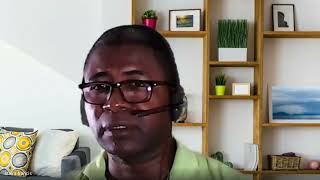
\includegraphics[scale=0.5]{images/stalin1.jpg}
    
    \caption[tutorias]{Compartiendo con los estudiantes y respondiendo dudas.}
    \label{fig:1}
\end{subfigure} \hspace{2cm}
\begin{subfigure}{0.45\linewidth}
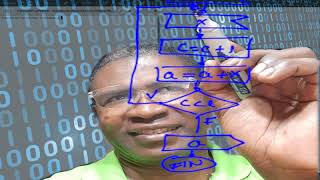
\includegraphics[scale=0.5]{images/stalin2.jpg}
    \caption[videotutorias]{Video tutoriales que refuerza el contenido de la guía de aprendizaje.}
    \label{fig:1}

\end{subfigure}


\caption{Evidencia de conexion y video tutorial}
\label{fig:xx}
\end{figure}



\vspace{2cm}

\begin{figure}[H]
\begin{subfigure}{0.45\textwidth}
    \centering
    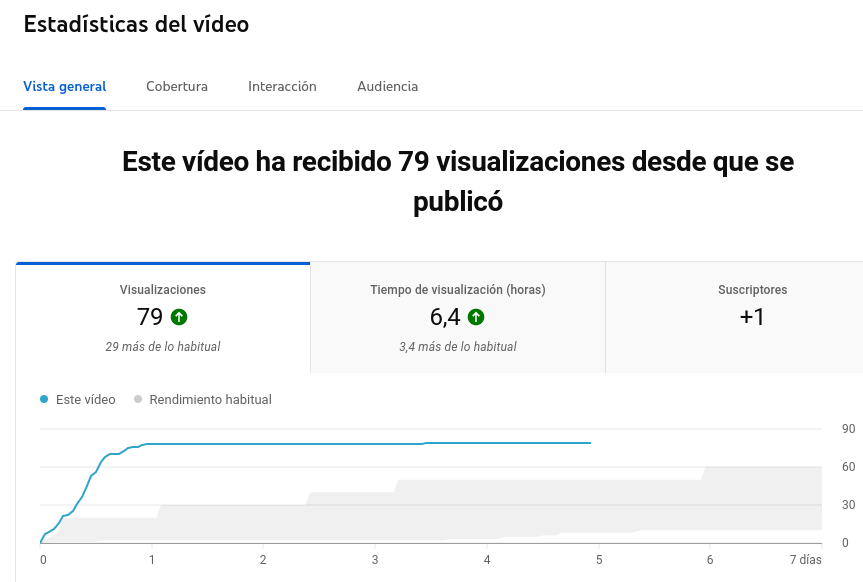
\includegraphics[scale=0.3]{images/estadistica1.png}
    
    \caption[tutorias]{Estadística de visualizaciones que ha tenido el vídeo.}
    \label{fig:1}
\end{subfigure} \hspace{2cm}
\begin{subfigure}{0.45\linewidth}
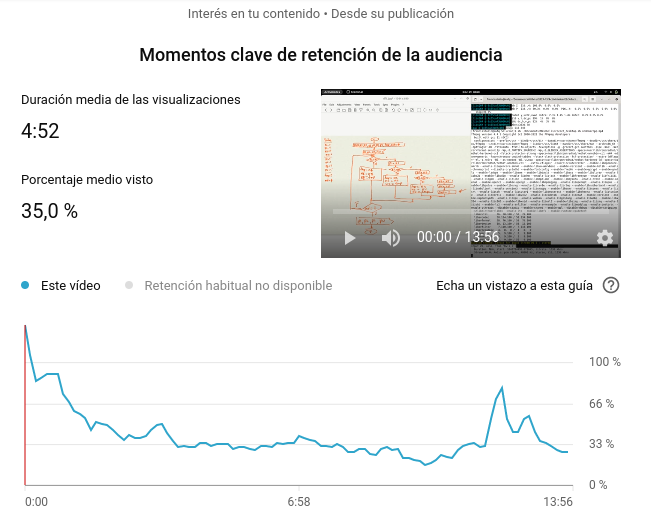
\includegraphics[scale=0.3]{images/estadistica2.png}
    \caption[videotutorias]{Estadística de retención de la audiencia.}
    \label{fig:1}

\end{subfigure}


\caption{Estadísticas que indican el nivel de visualización del los video tutoriales en youtube.}
\label{fig:xx}
\end{figure}




\section{Minería de datos}
\label{sec:procesamiento-de-la}
Los datos fueron obtenidos de los archivos  pdf que permite imprimir el sistema SIAC de la UTLVTE; para poder manipular los datos fue necesario convertir el archivo  pdf a formato texto, para este efecto se ejecuta  desde la linea de comando en linux la siguiente instrucción:\\


\begin{lstlisting}[language=bash]
  $ pdftotext -layout -eol unix pdf-entrada.pdf
\end{lstlisting}

\vspace{0.5cm}
Este comando arrojo un archivo tipo texto, el cual mediante el editor \textbf{vim} y  utilizando \textbf{expresiones regulares}, se lo convirtio en formato  cvs para poder ser cargado y analizado en la herrameinta R.\\

Alguna de las expresiones regulares fueron:\\
Para eliminar las linea en blanco

\begin{lstlisting}[language=vim]
  :%s/^\s\{2,\}\([0-9]\)/\1/g
\end{lstlisting}

Para separar los elementos con coma, reemplazando los espacia vacios: \\

\begin{lstlisting}[language=vim]
  :%s/\([0-9 a-z A-Z]\)\s\{1,\}/\1,/g
\end{lstlisting}






Luego de conseguir el archivo en formato csv, se utiliza el programa R. con el cual se cargo los datos como dataframe utilizando el siguiente comando:\\

\begin{lstlisting}[language=R]
pa <-read,table(``pa.csv'',head=TRUE,sep='','')
\end{lstlisting}

\vspace{0.5cm}

Luego de cargar el dataframe se procede a generar los histogramas con el siguiente comando ejecutado para cada columna:\\

hist(pa\$B1,breaks=50)


\vspace{0.5cm}
El gráfico del histograma que se analiza aquí,  permite saber la cantidad de estudiantes que han obtenido una calificación en el rango del (0-10). 

\section{Temas y Actividades cubiertos en el ciclo}
\label{sec:actividadades}


\begin{tabular}[H]{lp{5cm}p{2cm}p{7cm}l}
  \hline
   &Temas&cump & Actividades & \\ \hline \hline
   & Bibliografía & & \\
  0 & Presentación&100\% & & \\
  1 & Introducción&100\% & Actividad B1: Creación de un video  explicativo  & \\
  2 & Introducción a linux con termux&100\% &Actividad-C1-1-ParticipaciónClases: Uso de comandos en  linux utilizando termux & \\
  3 & Creación de archivos con vim &100\%& Actividad-C1-2-ParticipaciónClases: Uso del paquete vim y clang utilizando termux & \\
  4 & Github y la programación colaborativa&100\% &Actividad-A1.-Programación colaborativa con Github & \\
  5 & Examen del primer parcial&100\% &Actividad-E1. Examen del Primer parcial  & \\
  6 & Análisis y Diseño de Software&100\% &Actividad-B2-1: Introducción al Diseño con Diagrama de Flujo & \\
  7 & Introducción  a la programación en C++&100\% &Actividad-B2-2: TALLER DE ANALISIS Y DISEÑO & \\
  8 & Estructura de selección&100\% & & \\
  9 & Estructura de repetició&100\%n &Actividad-C2.- Diagrama de Flujo y Códificación en C++ & \\
  10 & Librerías y funciones&100\% &Actividad-A2.- Diagrama de Flujo y Código en C++ de proglemas tipo examen  & \\
  11 & Introducción a POO&100\% & & \\
  12 & Examen del segundo parcial&100\% &Actividad-E2. Examen 2do Parcial & \\
  13 & Recuperación&100\%&Actividad-S2.- Examen de Recuperación   &  \\ \hline \hline
  
\end{tabular}



\section{Cumplimiento de actividades}
\label{sec:cuml-de-activv}

\subsection{Actividad B1}
\label{sec:acctiviidad-b1}
Esta actividad que tenia un peso de 1.5/10, se observa que un porcentaje considerable de estudiantes no lo presentaron, pero también se demuestra que un porcentaje considerable si lo pudo realizar y sacarse la máxima calificación.\\


\begin{minipage}[h]{0.45\linewidth}
Paralelo-A

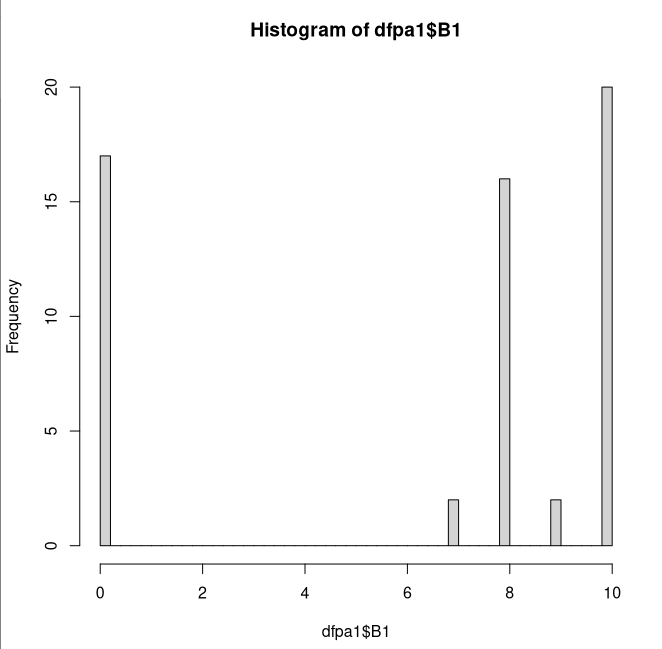
\includegraphics[scale=0.3]{images/histoB1.png}
\end{minipage}
\begin{minipage}[h]{0.45\linewidth}
Paralelo-B

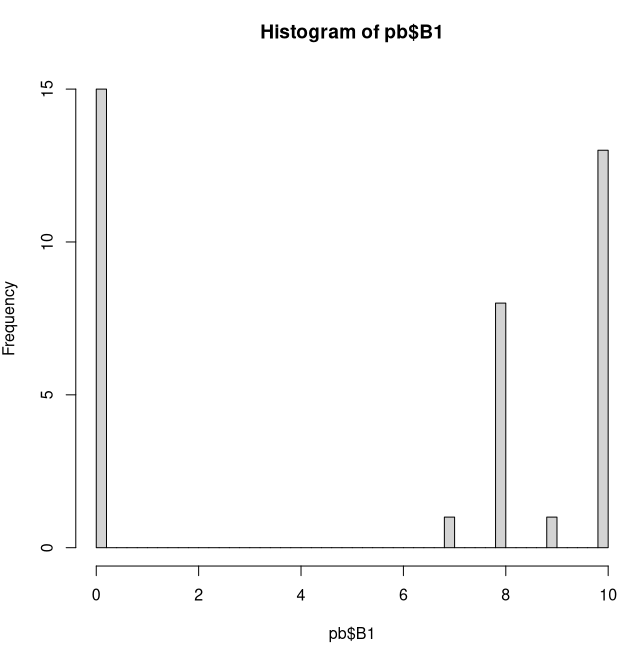
\includegraphics[scale=0.3]{images/histo-PB-B1.png}
\end{minipage}



\subsection{Actividad C1}
\label{sec:acctiviidad-c1}
Esta actividad tuvo un peso de 3/10, pero por el abandono que tuvieron algunos en la actividad anterior no pudieron realizarla, aunque también se observa que hubieron estudiantes que sacaron la máxima nota lo que demuestra que si era realizable.\\



\begin{minipage}[h]{0.45\linewidth}
  Paralelo-A.
  
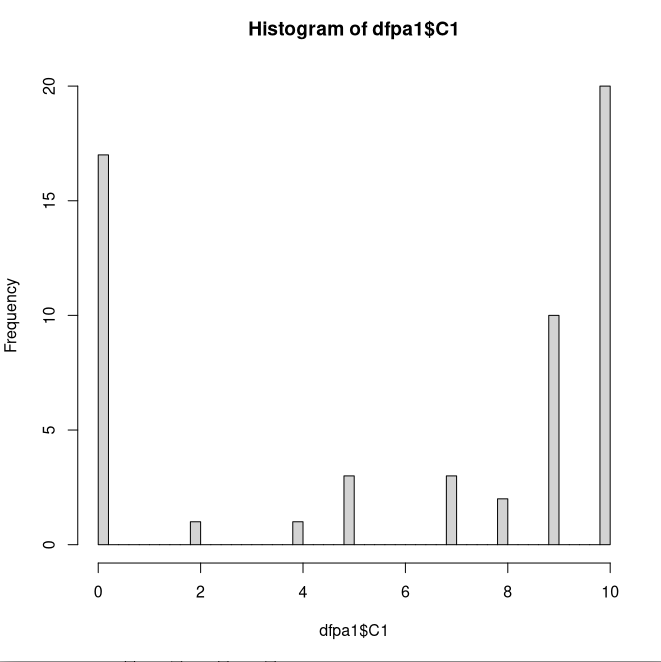
\includegraphics[scale=0.3]{images/histoC1.png}
\end{minipage}
\begin{minipage}[h]{0.45\linewidth}
  Paralelo-B.
  
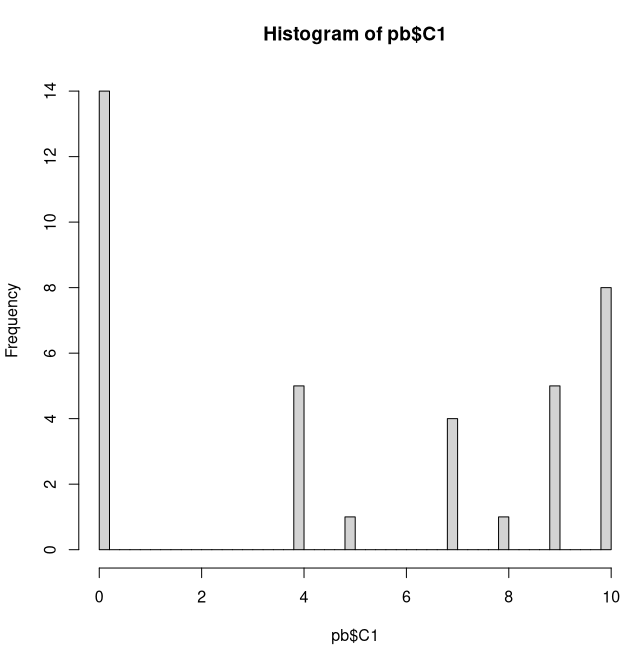
\includegraphics[scale=0.3]{images/histo-PB-C1.png}
\end{minipage}






\subsection{Actividad A1}
\label{sec:acctiviidad-A1}
Se muestra que la actividad fue realizable ya que la mayoria pudo obtener la maxima calificion de 10. esto se lo logro con el prograam R.  y el comando.\\


\begin{minipage}[h]{0.45\linewidth}
Paralelo-A

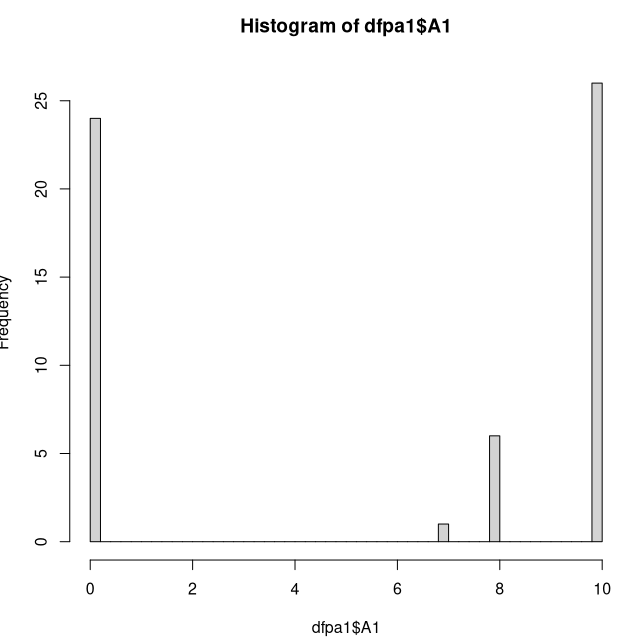
\includegraphics[scale=0.3]{images/histoA1.png}
\end{minipage}
\begin{minipage}[h]{0.45\linewidth}
Paralelo-B.

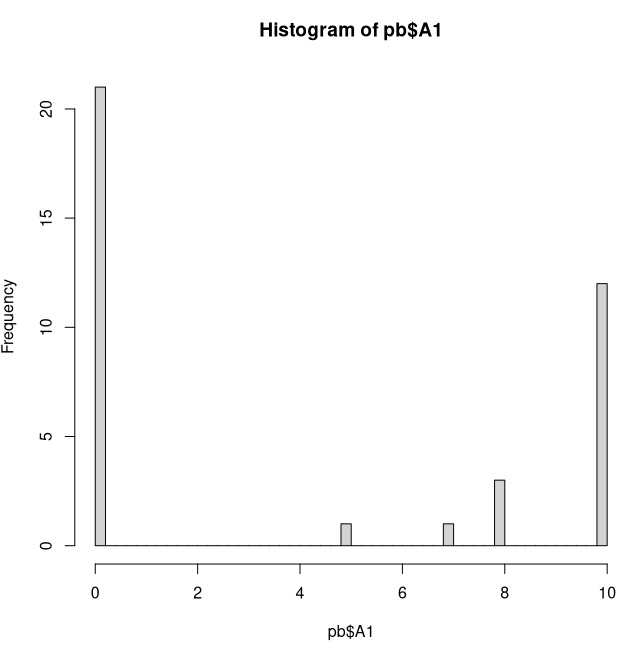
\includegraphics[scale=0.3]{images/histo-PB-A1.png}
\end{minipage}




\subsection{Actividad E1}
\label{sec:acctiviidad-e1}
Por el mejor desempleño en las actividades de aprendizaje en el paralelo A se ve reflejado en el Examen del primer parcial.\\



\begin{minipage}[h]{0.45\linewidth}
Paralelo-A.

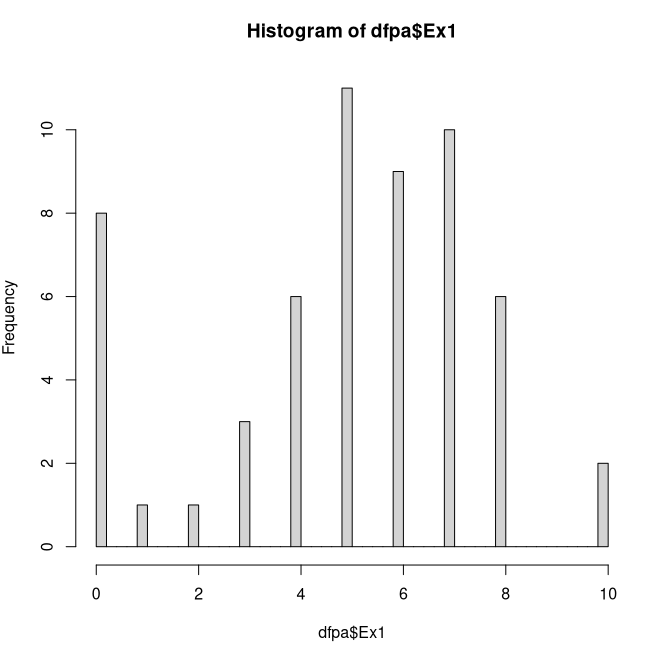
\includegraphics[scale=0.3]{images/histoEx1.png}
\end{minipage}
\begin{minipage}[h]{0.45\linewidth}
Paralelo-B.

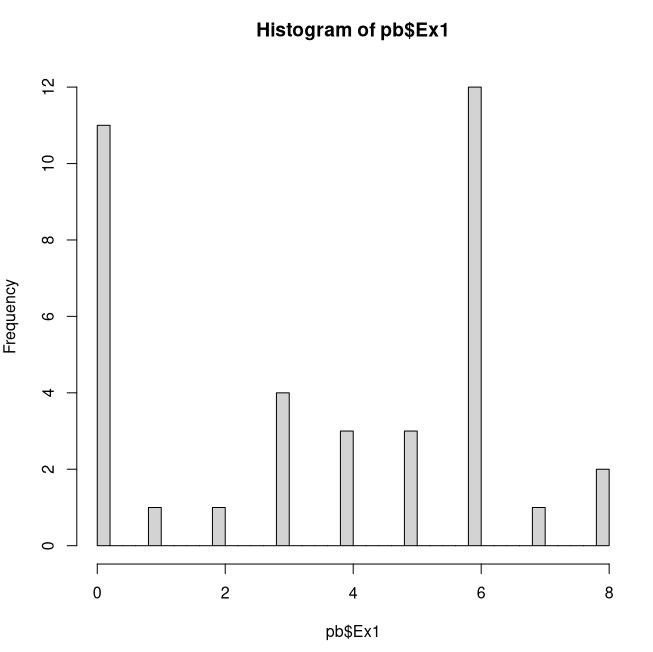
\includegraphics[scale=0.3]{images/histo-PB-Ex1.png}
\end{minipage}





\subsection{Actividad B2}
\label{sec:actividad-b2}
Esta actividad del segundo parcial son ya más complejas por eso se observa que menos estudiantes llegan a las máximas notas, pero el hecho que si existan notas altas, indica que si era posible realizarla.\\






\begin{minipage}[h]{0.45\linewidth}
  Paralelo-A
  .

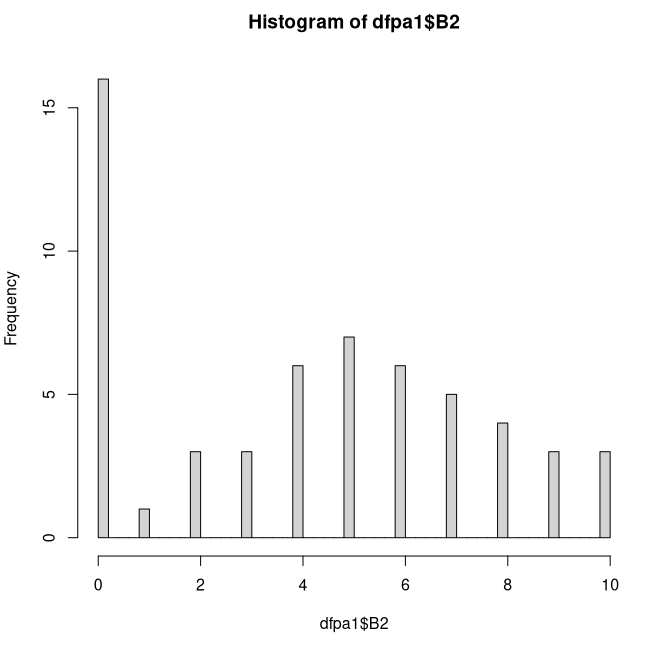
\includegraphics[scale=0.3]{images/histoB2.png}
\end{minipage}
\begin{minipage}[h]{0.45\linewidth}
paralelo-B

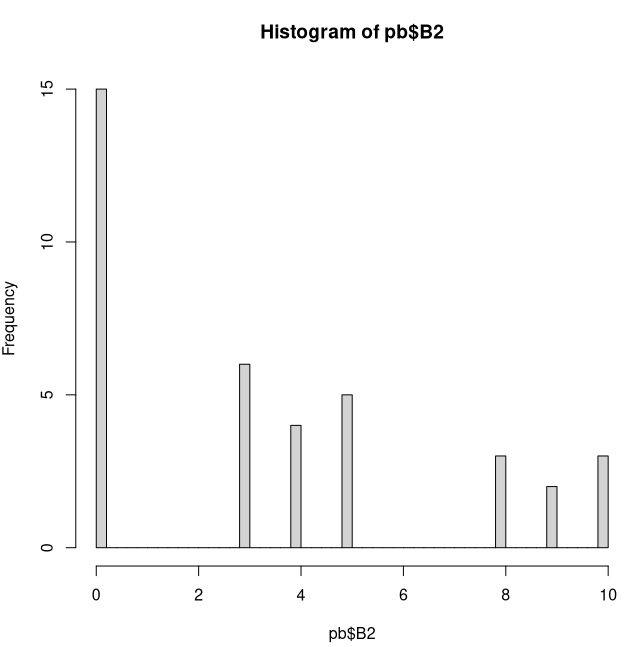
\includegraphics[scale=0.3]{images/histo-PB-B2.png}
\end{minipage}


\subsection{Actividad C2}
\label{sec:actividad-c2}
En esta actividad solo se puede ver que se mantiene el patrón de la actividad anterior donde el paralelo A demuestra un mayor cumplimiento que el paralelo B, aun así se observa un alto nivel de estudiantes que no presentan las actividades.\\



\begin{minipage}[h]{0.45\linewidth}
Paralelo-A.

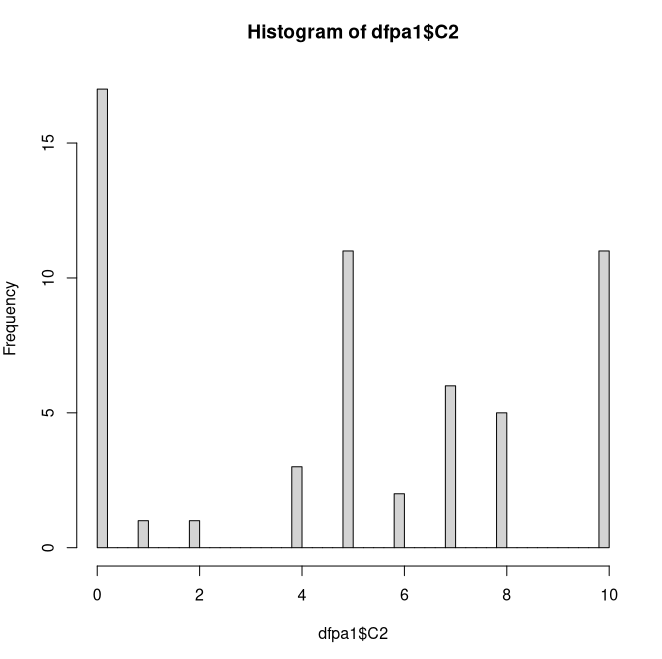
\includegraphics[scale=0.3]{images/histoC2.png}
\end{minipage}
\begin{minipage}[h]{0.45\linewidth}
Paralelo-B.

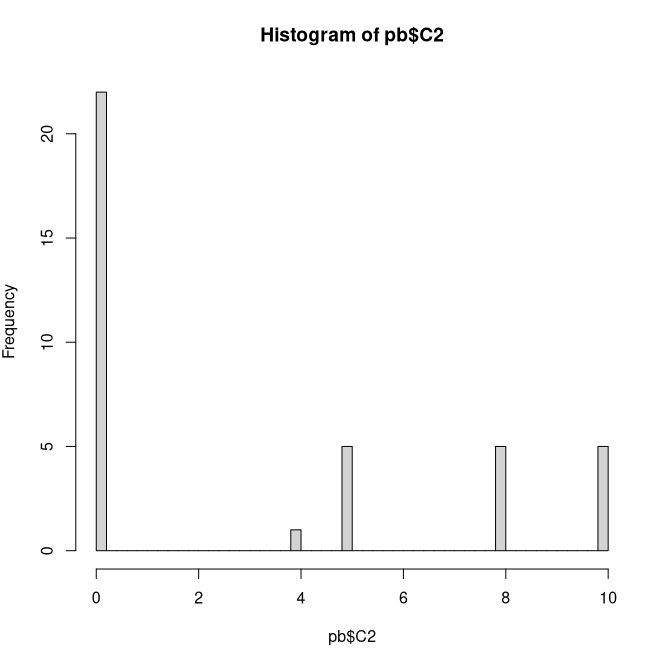
\includegraphics[scale=0.3]{images/histo-PB-C2.png}
\end{minipage}





\subsection{Actividad A2}
\label{sec:actividad-A2}
Esta actividad que es en equipo, se observa que un gran porcentaje de estudiantes no la entrego en los dos paralelos, pero también se puede observar que en el paralelo B, más estudiantes obtuvieron la máxima nota de 10 que en el paralelo A.\\



\begin{minipage}[h]{0.45\linewidth}
Paralelo-A.

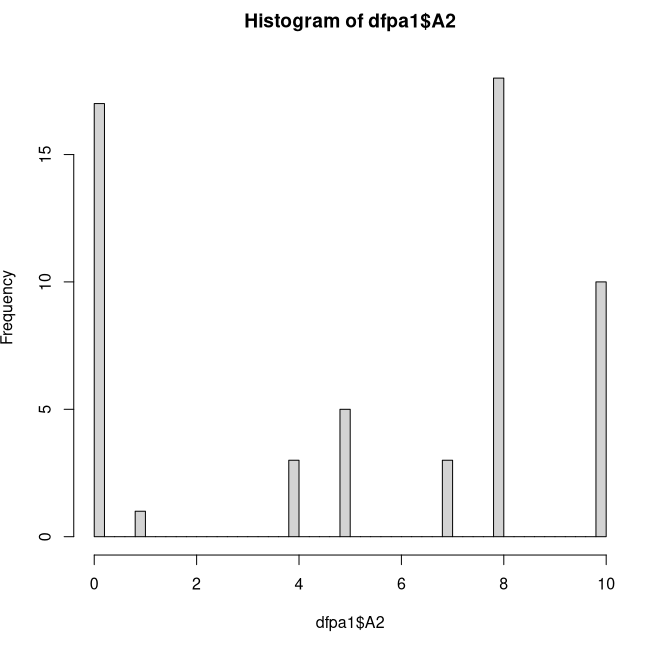
\includegraphics[scale=0.3]{images/histoA2.png}
\end{minipage}
\begin{minipage}[h]{0.45\linewidth}
Paralelo-B.

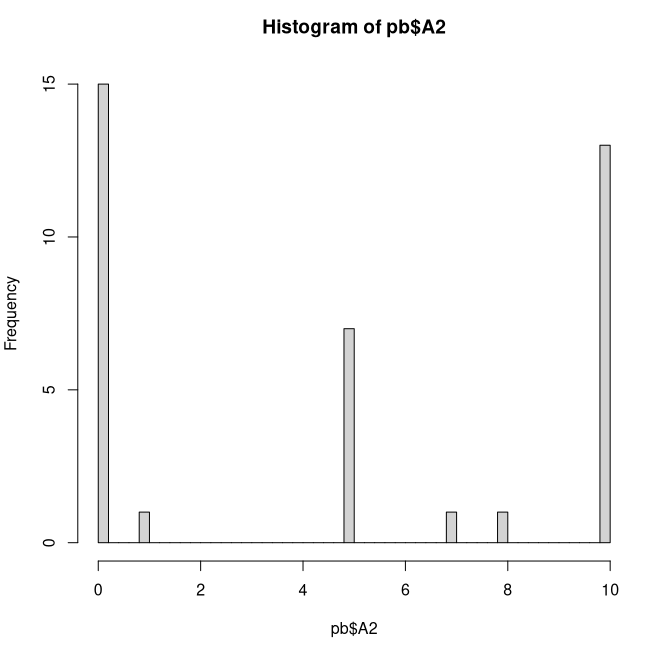
\includegraphics[scale=0.3]{images/histo-PB-A2.png}
\end{minipage}





\subsection{Actividad E2}
\label{sec:actividad-E2}
En el examen del segundo parcial más estudiantes en el paralelo B, obtuvieron la máxima calificación del 10, mientras que en el paralelo A, solo llegaron hasta 8.\\


\begin{minipage}[h]{0.45\linewidth}
Paralelo-A.

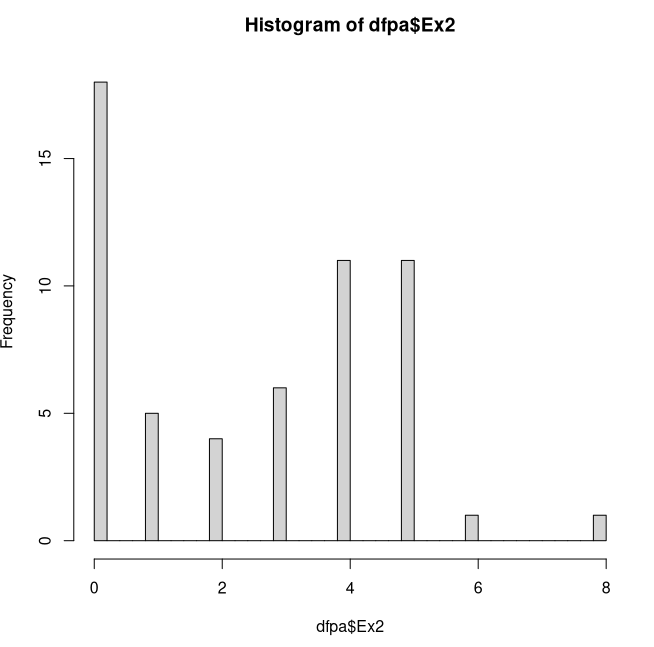
\includegraphics[scale=0.3]{images/histoEx2.png}
\end{minipage}
\begin{minipage}[h]{0.45\linewidth}
Paralelo-B.

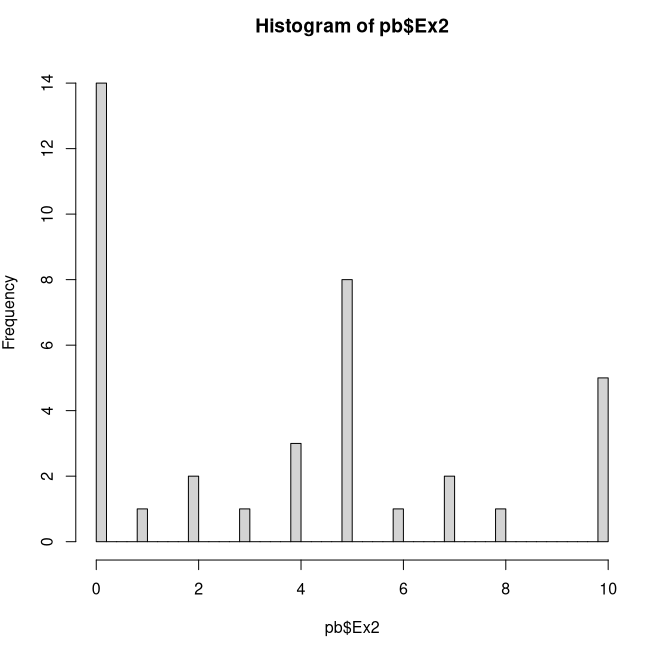
\includegraphics[scale=0.3]{images/histo-PB-Ex2.png}
\end{minipage}



\subsection{Promedio  Final}
\label{sec:actividad-E2}
El promedio Final muestra el resultado de las actividad de aprendizaje, se observa que en el paralelo B, más estudiantes tiene bajas notas que el paralelo A, pero también más estudiantes en el paralelo B obtuvieron la máxima nota que en el paralelo A.\\




\begin{minipage}[h]{0.45\linewidth}
Paralelo-A.

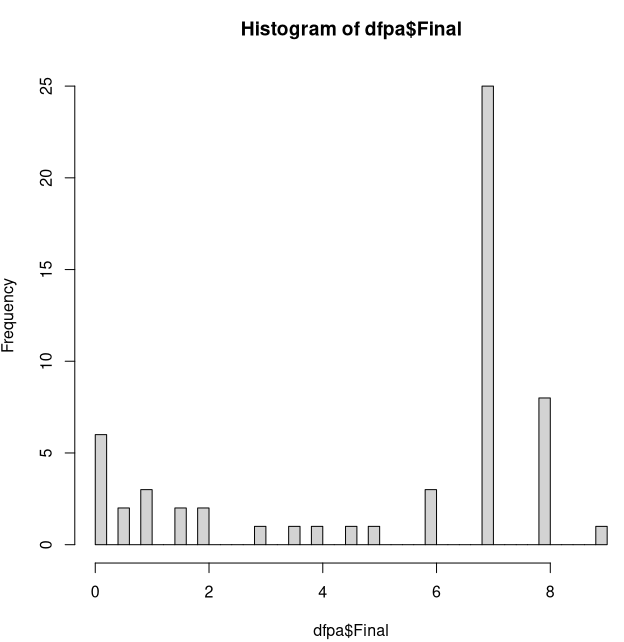
\includegraphics[scale=0.3]{images/histoFinal.png}
\end{minipage}
\begin{minipage}[h]{0.45\linewidth}
Paralelo-B.

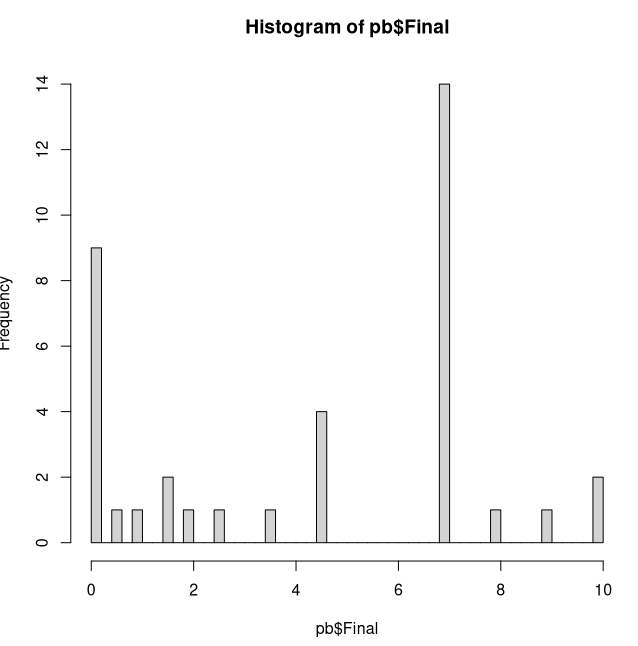
\includegraphics[scale=0.3]{images/histo-PB-Final.png}
\end{minipage}


\section{Resumen}
\label{sec:resumen}


\begin{tabular}[h]{|l|r|r|r|r|}
  \hline
  Paralelos & \#estudiantes & DESERTORES & REPROBADOS & APROBADOS \\ \hline \hline
  A         & 57  & 16     &    16+7=23  & 34  \\
  B         & 38  & 14     &  14+7=21 &   17      \\ \hline
\end{tabular}

\section{Conclusión}
\label{sec:conclusion}

\begin{enumerate}
\item La mayoría de los estudiantes que reprueban la asignatura ha
  sido por deserción (20\% paralelo A, 37\% paralelo B).

  
\item La cantidad de  estudiantes reprobados por no obtener el puntaje mínimo requerido fue bastante baja(12\% paralelo A, 18\% en el paralelo B).
  
\item El porcentaje de estudiantes aprobados fue bastante alta(60\% en el paralelo A, 45\% en el paralelo B).
  
\end{enumerate}

\bibliographystyle{apacite}

\setlength{\bibleftmargin}{.125in}
\setlength{\bibindent}{-\bibleftmargin}
\bibliography{Referencia}

\newpage
\vspace{0.3cm}


\noindent \textbf{Fecha de elaboración:} 3 de enero del 2021. \\
\textbf{Autor del Informe: } Ing. Staln Francis Quinde. \\
\textbf{Revisión del Informe: } Ing. Staln Francis Quinde. \\

\vspace{4cm}

\vspace{3cm}
\begin{center}
\begin{tabular}[H]{m{8cm}lm{8cm}}
  \rule{7cm}{0.4pt}& &\rule{7cm}{0.4pt} \\
  \makecell[c]{Ing. Stalin Francis Ms.c\\\textbf{ DOCENTE}}  & &\makecell[c]{Ing. Jonathan Cardenas  MSc. \\ \textbf{COORDINADOR DE ÁREA ACADÉMICA} \\ \textbf{DE PROGRAMACIÓN}} \\ 
\end{tabular}
\end{center}

\vspace{3cm}
\begin{center}

\begin{tabular}[H]{m{8cm}lm{8cm}}
  
  \rule{7cm}{0.4pt}&  & \\
  \makecell[c]{Ing. Baster Estupiñan Ortiz, MSc. \\ \textbf{DIRECTOR DE CARRERA DE INGENIERÍA} \\ \textbf{EN TECNOLOGÍÁ DE LA INFORMACIÓN}} & &  
\end{tabular}
\end{center}





\end{document}

%%% Local Variables:
%%% mode: latex
%%% TeX-master: t
%%% End:
